The Jefferson Lab EIC is based on a ring-ring collider design with a high repetition rate, strong focusing, and low emittance.  The baseline design results in luminosity approaching $10^{-34}$ cm$^{-2}$ s$^{-1}$ at each interaction point and the figure-8 design produces over 70\% polarization for both electron and ion beams.  The design permits two full-acceptance detectors integrated with the accelerator in the interaction regions.  [Pilat, 2017]

\begin{figure}
	\centering
	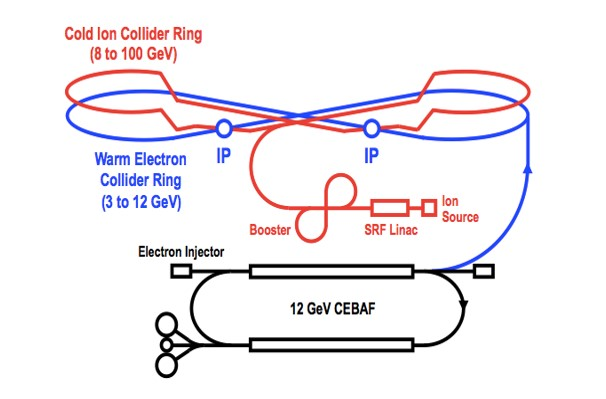
\includegraphics[width=.75\textwidth]{../../img/jleic_schematic.jpg}
	\caption{Schematic of the Jefferson Lab EIC}
	\label{fig:jleic1}
\end{figure}

Table 1 summarizes some of the relevant design parameters for the machine.  The JLEIC machine is unique, and thus background rates and mitigation choices will be specific to the machine design.  While much can be learned from previous machine experiences, the JLEIC configuration will be the first of its kind and thorough background studies with its specific parameters must be completed.

\begin{center}
	\begin{tabular}{ l l l l } 
		\multicolumn{4}{c}{JLEIC Parameters}  \\ 
		\hline \hline
		& & p & e\\
		\hline
		Beam energy & GeV & 100 & 5 \\ 
		Collision frequency & MHz& \multicolumn{2}{c}{476}\\ 
		Particles per bunch & $10^10$ & 0.66 & 3.9\\
		Beam current & A & 0.5 & 3 \\
		Polarization &  & \textgreater70\% & \textgreater70\%\\
		Bunch length, rms & cm & 1 & 1.2 \\
		Norm. emittance, x/y& $\mu$m & 1/0.5 & 144/72  \\
		x/y $\beta^*$ & cm &4/2 & 2.6/1.3\\
		Vert. beam-beam param.& & 0.006 & 0.014\\
		Laslett tune shift & & 0.01 & Small \\
		Detector space, up/down & m & 3.6/7 & 2.4/1.6 \\
		Hourglass (HG)reduction & & \multicolumn{2}{c}{0.88}\\
		Lumi./IP, w/ HG, $\mathbf{10^{33}}$ & cm$^{-2}$ s$^{-1}$ & \multicolumn{2}{c}{4.6} \\
		\hline
	\end{tabular}
\end{center}

\subsection{Detector Region}

The full-acceptance detector region has been placed far from the electron arc exit to minimize the synchrotron radiation background, and close to the ion arc exit to minimize the hadronic background from ion beam scattering on residual gas.  While long, straight section of machine lattice minimizes the synchrotron radiation from magnet bending, it is possible that electron beam scattering on beamline gas interactions could generate enough synchrotron radiation to negatively impact the detectors.  A small upstream chicane has been proposed to mitigate this effect.  The quantity and distribution of synchrotron radiation from beam-gas interaction must be evaluated, along with the effectiveness of a chicane.  Such a study is within the scope of this proposal.  
\begin{figure}
	\centering
	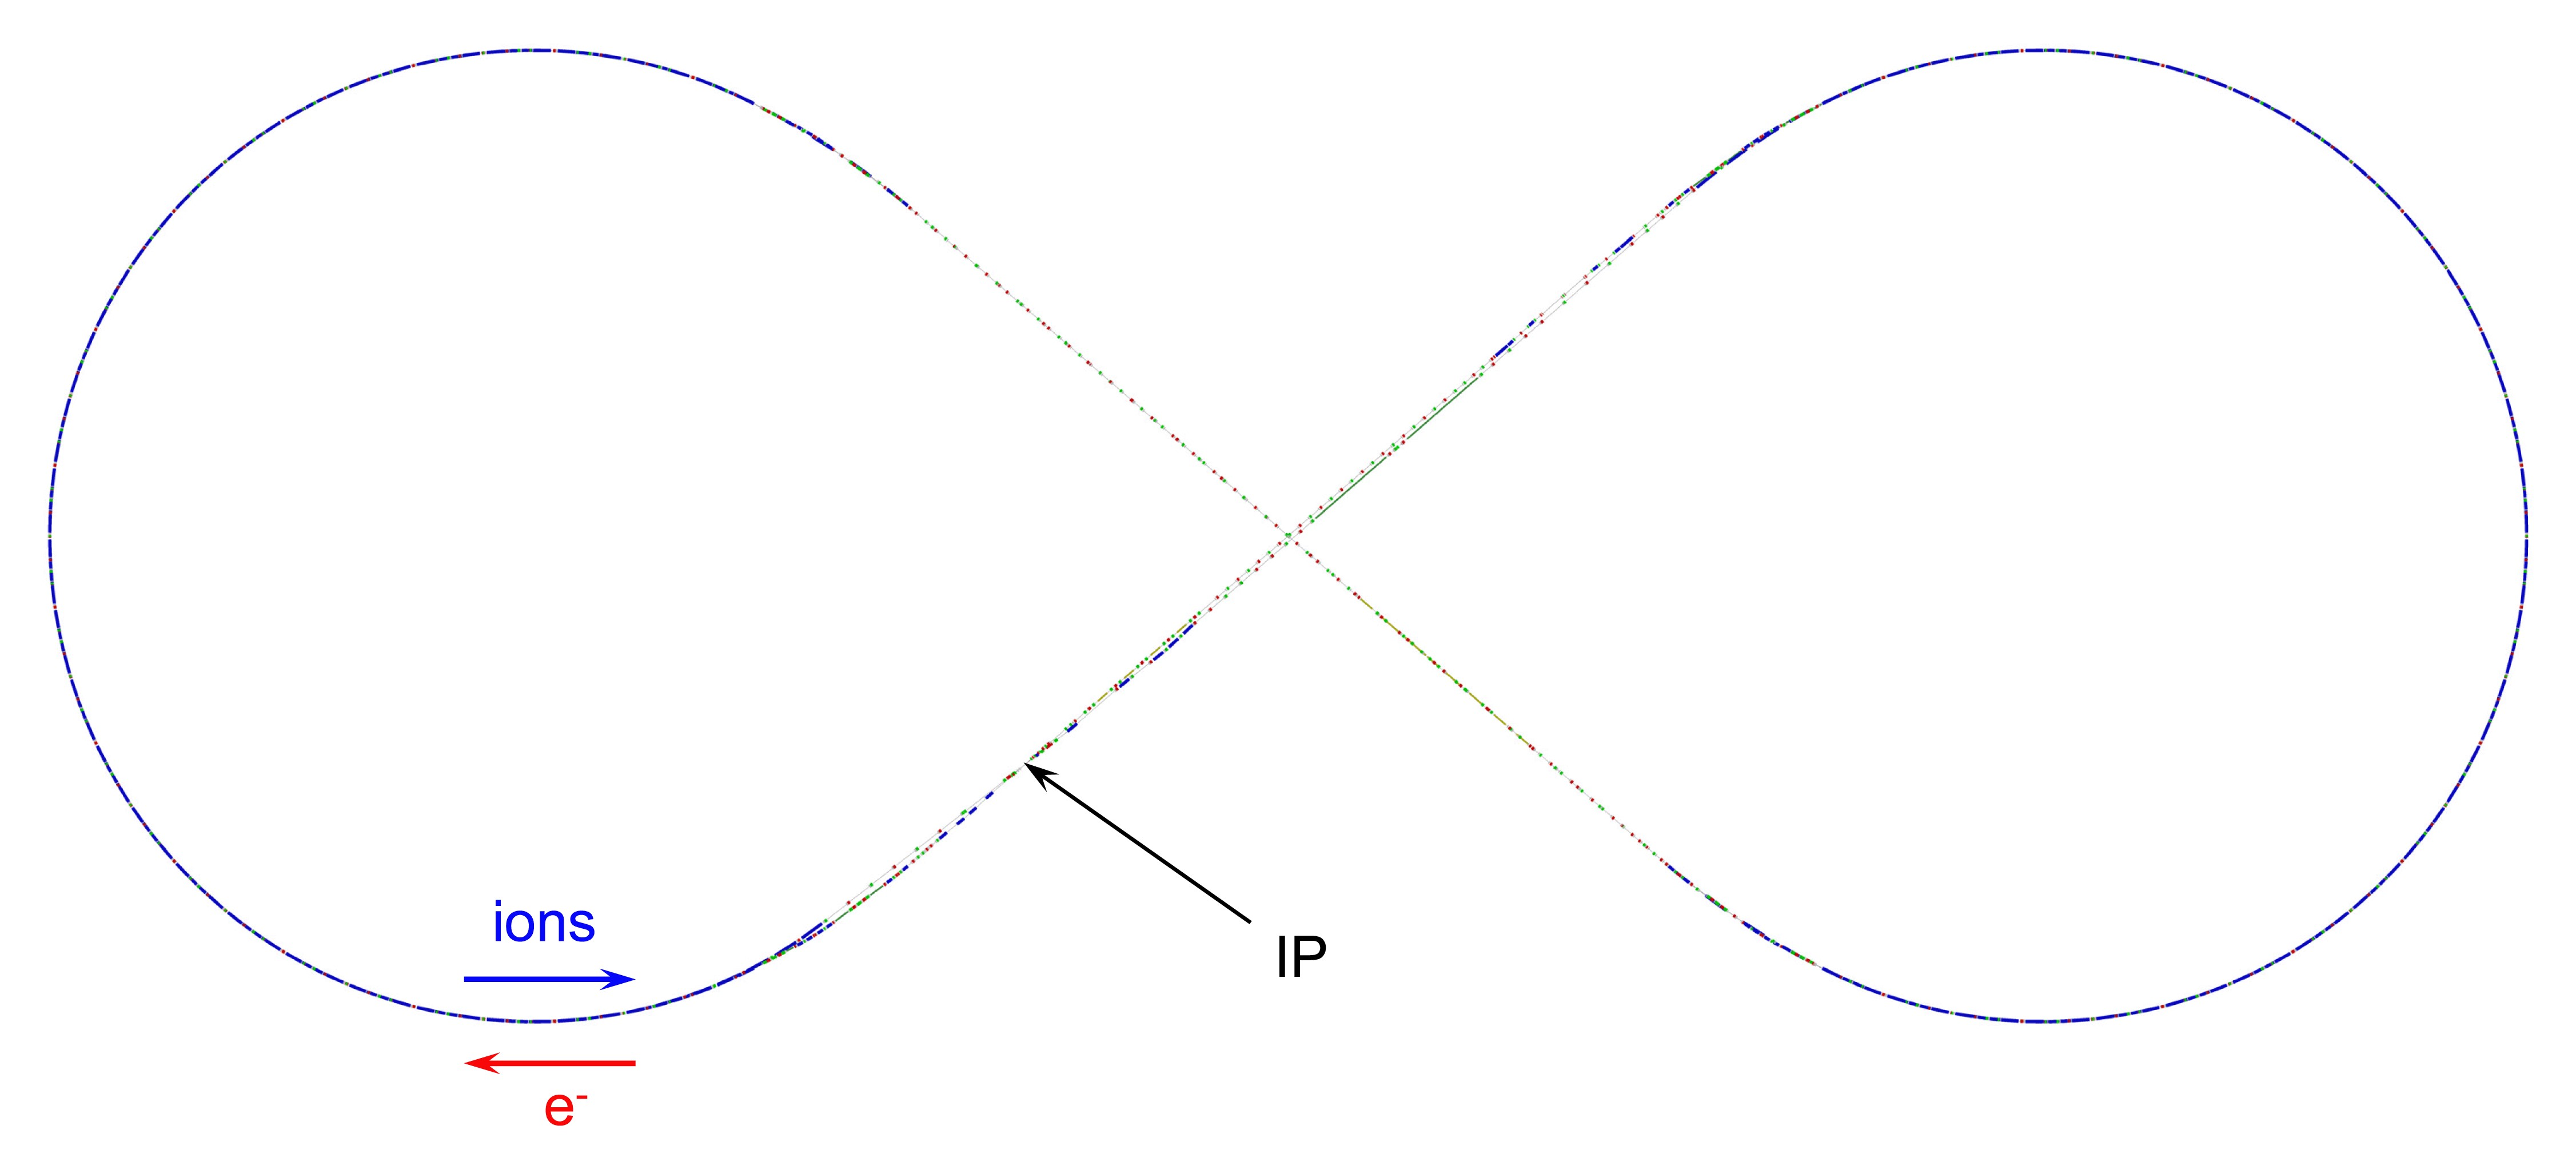
\includegraphics[width=.75\textwidth]{../../img/collider_rings_layout.jpg}
	\caption{Collider rings' Layout.}
	\label{fig:jleic2}
\end{figure}
%edit image with curly brackets to indicate electron and ion beam components also chican Mike mentioned possibly putting in?
\begin{figure}[h!]
	\centering
	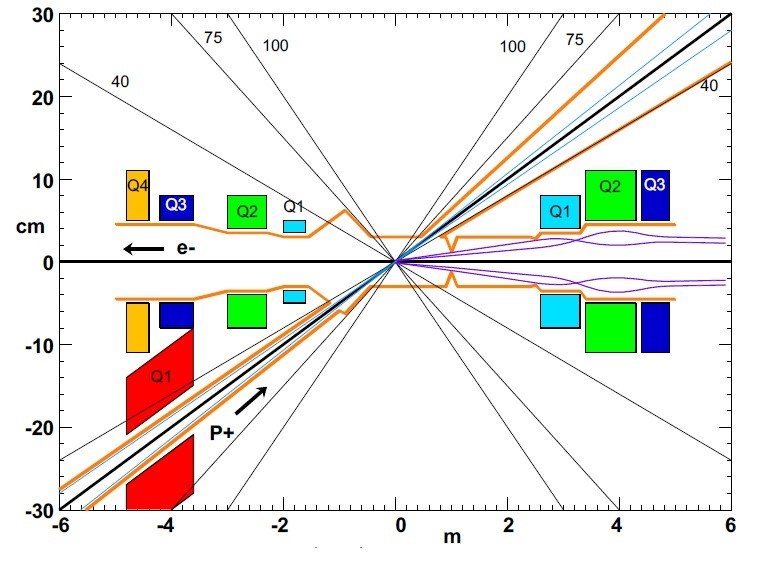
\includegraphics[width=.75\textwidth]{../../img/new_beam_pipe.jpg}
	\caption{Schematic of the JLEIC interaction region beam pipe design.}
	\label{fig:jleic3}
\end{figure}

\begin{figure}[t]
	\centering
	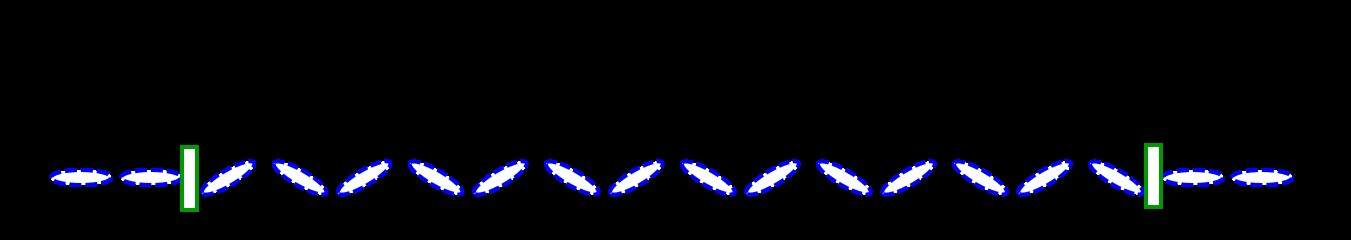
\includegraphics[width=.75\textwidth]{../../img/crab_bunch_profile.jpg}
	\caption{Evolution of the horizontal bunch profile between the crab cavities.}
	\label{fig:jleic4}
\end{figure}

\subsection{Interaction Region Beam Pipe}
The current JLEIC beam pipe design incorporates several features to minimize background and interaction with beampipe material.  It utiliizes a 50 mrad crossing angle for quick beam separation, and incorporates masking within the electron pipe to collimate synchrotron radiation before reaching the IP.  The current design utilizes gold coatings and water cooling, and a beam stay-clear of 10$\sigma$ + 5 mm. This study proposes to develop the code needed to implement the beam pipe design in the simulation tools such as GEMC and Molflow+ and study the impact of design choices on the quantities of background delivered to the detectors.  While the beam crossing angle is specific to the JLEIC machine, the beam pipe design and background mitigation choices is of generic interest to both Jefferson and Brookhaven designs.
%insert images of newest beampipe design


\subsection{Bunch Tilt}
The 50 mrad crossing angle provides quick beam separation, minimizing unwanted beam-beam interactions and subsequent background.  The JLEIC design incorporates a local compensation scheme using SRF crab cavities to restore head-on collisions and compensate for the luminosity loss due to the nonzero crossing angle.  

This bunch tilt in the horizontal plane may create hadronic and leptonic background fluctuations which need to be considered.  Both Jefferson and Brookhaven designs incorporate crab cavities, and a quantitative understanding of the background fluctuations is of mutual benefit. 





